\documentclass[11pt]{article}
\usepackage{amsmath, amssymb, amsthm}
\usepackage{geometry}
\usepackage{booktabs}
\usepackage{multirow}
\usepackage{hyperref}
\usepackage{xcolor}
\usepackage{microtype}
\usepackage{listings}
\usepackage{graphicx}
\geometry{margin=1in}

\theoremstyle{remark}
\newtheorem{remark}{Remark}

\lstset{basicstyle=\ttfamily\small, breaklines=true, frame=single}

\title{What Governs the Adaptive Regime?\\
       Testing a Dimensionless Ratio in Viability-Constrained Memory Systems}
\author{VCSM Theory Series --- Paper 9}
\date{2026}

\begin{document}
\maketitle

\begin{abstract}
Papers~7 and~8 showed that the adaptive window of a VCML substrate sits at
$\nu^* \approx 0.001$, invariant to propagation strength $\kappa$ and to the
consolidation parameters SS and FIELD\_ALPHA within their operational ranges.
An order-of-magnitude balance equation identified the wave input dynamics as the
likely controlling factor. Paper~9 asks the follow-on question:
\emph{does a single dimensionless ratio $\Xi = \nu \cdot (N/4) \cdot
2\,\mathtt{WAVE\_DUR}/\mathtt{WR}$ govern the window location?} We test this
with two experiments: a WAVE\_DUR sweep at fixed WR (testing $\nu^* \propto
1/\mathtt{WAVE\_DUR}$) and a ratio-collapse test holding $R = \mathtt{WR}/
\mathtt{WAVE\_DUR}$ constant while varying each individually. The Xi collapse is
\emph{not confirmed}: $\Xi^*$ varies across conditions (0.03 to 2.5 in Exp~1;
0.19 to 0.625 in Exp~2), and the ratio collapse fails. The failure reveals that
WR and WAVE\_DUR have independent effects on $\nu^*$ beyond their ratio, with
absolute WR setting the perturbation load $P_{\text{pert}} = 1 - e^{-WR/2}$
and absolute WAVE\_DUR setting the consolidation probability $P_{\text{calm}}$.
The regime boundary is governed by at least two dimensionless quantities, not
one. This is a more complete picture than Paper~8's balance equation provides,
and it identifies the specific quantities a better theoretical model must account for.
\end{abstract}

% ============================================================
\section{Introduction}

Paper~8 (Empirical Turnover Invariance) showed that $\nu^* \approx 0.001$ is
stable across propagation and consolidation parameters, and proposed the following
order-of-magnitude balance equation for $\nu^*$:
\begin{equation}
  \nu^*_{\text{pred}} \;=\; \frac{\mathtt{WR}}{2 \cdot \mathtt{WAVE\_DUR}
    \cdot N_{\text{act}}/4}
  \label{eq:balance}
\end{equation}
Paper~8 explicitly noted this was a \emph{post-hoc consistency check}, not a
predictive law. Paper~9 converts it into a test: if Eq.~\eqref{eq:balance}
is the correct balance, then the adaptive regime is governed by the
dimensionless ratio:
\begin{equation}
  \Xi \;=\; \frac{\nu}{\nu^*_{\text{pred}}} \;=\;
    \frac{\nu \cdot 2 \cdot \mathtt{WAVE\_DUR} \cdot N_{\text{act}}/4}{\mathtt{WR}}
  \label{eq:xi}
\end{equation}
and all $\mathtt{sg4}$-vs.-$\nu$ curves, when re-plotted as $\mathtt{sg4}$-vs.-$\Xi$,
should collapse onto a single peak at $\Xi^* \approx$ constant.

Two experiments test this:
\begin{enumerate}
  \item \textbf{WAVE\_DUR sweep} (Exp~1): fix WR, vary WAVE\_DUR. Prediction:
    $\nu^* \propto 1/\mathtt{WAVE\_DUR}$; $\Xi^*$ constant.
  \item \textbf{Ratio collapse} (Exp~2): fix $R = \mathtt{WR}/\mathtt{WAVE\_DUR} =
    0.32$, vary WR and WAVE\_DUR jointly. Prediction: $\nu^*$ identical across
    all pairs; $\Xi^*$ constant.
\end{enumerate}

Both predictions fail. Section~\ref{sec:interp} interprets the failure and
identifies what the balance equation is missing.

\subsection{Background: Two Rates Governing Consolidation}

From the VCSM update rule, two distinct rates set the consolidation environment:

\begin{itemize}
  \item \textbf{Wave launch rate} $R = \mathtt{WR}/\mathtt{WAVE\_DUR}$: the
    expected number of new wave events per step per side. Controls how often new
    perturbation bursts arrive. Appears in the balance equation numerator.
  \item \textbf{Perturbation load} $P_{\text{pert}}(WR) = 1 - e^{-WR/2}$: the
    fraction of steps a site is perturbed by at least one active wave. Depends on
    absolute WR via the expected overlap of simultaneous active waves ($\approx WR/2$).
    Does \emph{not} appear in the balance equation.
  \item \textbf{Consolidation probability} $P_{\text{calm}} \approx
    (1 - R/2)^{SS + \mathtt{WAVE\_DUR} - 1}$: probability of achieving a calm
    streak $\geq SS$. Depends on both $R$ and absolute WAVE\_DUR.
\end{itemize}

The balance equation uses only $R$ and omits $P_{\text{pert}}$ and the
WAVE\_DUR contribution to $P_{\text{calm}}$. These omissions predict the
experimental outcomes.

% ============================================================
\section{Shared Protocol}

All experiments use the Paper~7 Exp1 base configuration, with WAVE\_DUR as a
new variable and an extended $\nu$ sweep for finer resolution.

\begin{center}
\begin{tabular}{ll}
\toprule
Parameter & Reference value \\
\midrule
Grid & $W=40$, $H=20$, $\mathtt{HALF}=20$, $N_{\text{act}}=400$ \\
$\mathtt{HS}$ & 2; $\mathtt{KAPPA}=0.020$; $\mathtt{SS}=10$; $\mathtt{FIELD\_ALPHA}=0.16$ \\
$\mathtt{STEPS}$ & 2000; $\mathtt{SHIFT}=1000$; Seeds = 5 \\
$\nu$ sweep & 12 values: $\{0.0001, 0.0002, 0.0003, 0.0005, 0.001, 0.002,$ \\
            & $\quad\quad\quad\quad\quad\quad 0.003, 0.005, 0.010, 0.020, 0.040, 0.080\}$ \\
\bottomrule
\end{tabular}
\end{center}

The 12-value sweep (vs.\ 9 in Papers~7--8) adds $\nu \in \{0.0002, 0.0005, 0.003\}$
for sub-factor-2 resolution around the expected $\nu^* \approx 0.001$.

% ============================================================
\section{Experiment 1: WAVE\_DUR Sweep}
\label{sec:exp1}

\subsection{Protocol}

$\mathtt{WAVE\_DUR} \in \{7, 15, 30, 60\}$, WR fixed at 4.8. $4 \times 12 \times
5 = 240$ runs.

\subsection{Results}

\begin{table}[h]
\centering
\caption{WAVE\_DUR sweep. $\nu^*_{\text{pred}} = 4.8/(2 \cdot \mathtt{WD} \cdot 100)$.
$\Xi^* = \nu^* \cdot 100 \cdot 2 \cdot \mathtt{WD}/4.8$.
sg4 profile: $\nu = 0.0001, 0.0002, \ldots, 0.080$ (12 values, boldface at $\nu^*$).}
\label{tab:exp1}
\begin{tabular}{r r r r r l}
\toprule
WD & $\nu^*_{\text{pred}}$ & $\nu^*$ & $\mathtt{sg4}^*$ & $\Xi^*$ & note \\
\midrule
 7 & 0.0034 & 0.0001 & 138.5 & 0.029 & over-perturbed; no adaptive peak \\
15 & 0.0016 & 0.0005 & 419.0 & 0.312 & reference; finer grid shifts argmax \\
30 & 0.0008 & 0.0005 & 561.7 & 0.625 & matches balance-equation prediction \\
60 & 0.0004 & 0.0010 & 432.6 & 2.500 & reversed; broad noisy profile \\
\bottomrule
\end{tabular}
\end{table}

\textbf{Result.} $\Xi^*$ is \emph{not} constant: it varies from 0.029
(WAVE\_DUR=7) to 2.5 (WAVE\_DUR=60), an $85\times$ range. The Xi collapse fails.

Three regimes are evident:
\begin{itemize}
  \item \textbf{WAVE\_DUR=7} (over-perturbed): With $R = 4.8/7 = 0.69$, the wave
    launch rate relative to wave duration is high, and $P_{\text{calm}}(SS=10)
    \approx (1-0.34)^{16} \approx 0.0006$. Almost no site achieves a calm streak
    of 10; $\mathtt{sg4}$ decreases monotonically with $\nu$, and the system
    lacks a true adaptive peak. This parallels the WR=9.6 collapse in Paper~8
    Experiment~4.

  \item \textbf{WAVE\_DUR=15, 30} (operational range): Both show clear adaptive
    peaks at $\nu^* = 0.0005$, with $\Xi^* = 0.312$ and $0.625$ respectively.
    The balance equation predicted $\nu^* \propto 1/\mathtt{WAVE\_DUR}$ (a 2$\times$
    shift from WD=15 to WD=30), but both argmax at the same grid point. The true
    peaks are in the range $0.0005$--$0.001$; the factor-2 shift is smaller than
    the grid resolution permits detecting at the argmax level.

  \item \textbf{WAVE\_DUR=60} (reversed): $\nu^* = 0.001$, \emph{higher} than
    WAVE\_DUR=30. The sg4 profile is broad and non-monotone around the peak
    ($\mathtt{sg4} = 261$ at $\nu = 0.0005$; $\mathtt{sg4} = 433$ at $\nu =
    0.001$), suggesting high variance at 5 seeds and possibly transient dynamics
    not resolved in 2000 steps for such infrequent perturbations.
\end{itemize}

% ============================================================
\section{Experiment 2: Ratio Collapse}
\label{sec:exp2}

\subsection{Protocol}

Three $(WR, \mathtt{WAVE\_DUR})$ pairs with $R = \mathtt{WR}/\mathtt{WAVE\_DUR}
= 0.32$ (reference value):

\begin{center}
\begin{tabular}{rrrrrr}
\toprule
WR & WD & $R$ & $\nu^*_{\text{pred}}$ & $P_{\text{pert}}(WR)$ & $P_{\text{calm}}$ \\
\midrule
1.6 &  5 & 0.32 & 0.0016 & 0.551 & 0.084 \\
4.8 & 15 & 0.32 & 0.0016 & 0.909 & 0.015 \\
9.6 & 30 & 0.32 & 0.0016 & 0.992 & 0.0013 \\
\bottomrule
\end{tabular}
\end{center}

Note that $\nu^*_{\text{pred}} = R/(N_{\text{act}}/2) = 0.0016$ is identical
for all three. However, $P_{\text{pert}}$ and $P_{\text{calm}}$ differ substantially.

\subsection{Results}

\begin{table}[h]
\centering
\caption{Ratio collapse test. Same $R = 0.32$; only absolute WR and WD differ.
If $R$ alone governs $\nu^*$, the $\nu^*$ column should be identical.}
\label{tab:exp2}
\begin{tabular}{r r r r r r}
\toprule
WR & WD & $\nu^*$ & $\mathtt{sg4}^*$ & $\Xi^*$ & $P_{\text{pert}}$ \\
\midrule
1.6 &  5 & 0.0010 & 206.1 & 0.625 & 0.55 \\
4.8 & 15 & 0.0005 & 419.0 & 0.312 & 0.91 \\
9.6 & 30 & 0.0003 & 402.7 & 0.188 & 0.99 \\
\bottomrule
\end{tabular}
\end{table}

\textbf{Result.} $\nu^*$ is \emph{not} constant across pairs with equal $R$:
it decreases from $0.001$ to $0.0005$ to $0.0003$ as WR grows from 1.6 to 9.6
(a 3$\times$ variation across the same $R$). $\Xi^*$ correspondingly varies
from 0.625 to 0.312 to 0.188. The ratio $R$ alone does not determine $\nu^*$.

The monotone decrease of $\nu^*$ with WR (at fixed $R$) correlates with the
monotone increase of $P_{\text{pert}}$: as WR grows, sites are perturbed a
greater fraction of the time (91\% at WR=4.8; 99\% at WR=9.6), increasing the
effective death rate above the nominal $\nu$. The balance condition is reached
at a lower nominal $\nu$ when the effective rate is already elevated by
perturbation-induced extra aging.

% ============================================================
\section{Figure: The Partial Collapse}

\begin{figure}[h]
\centering
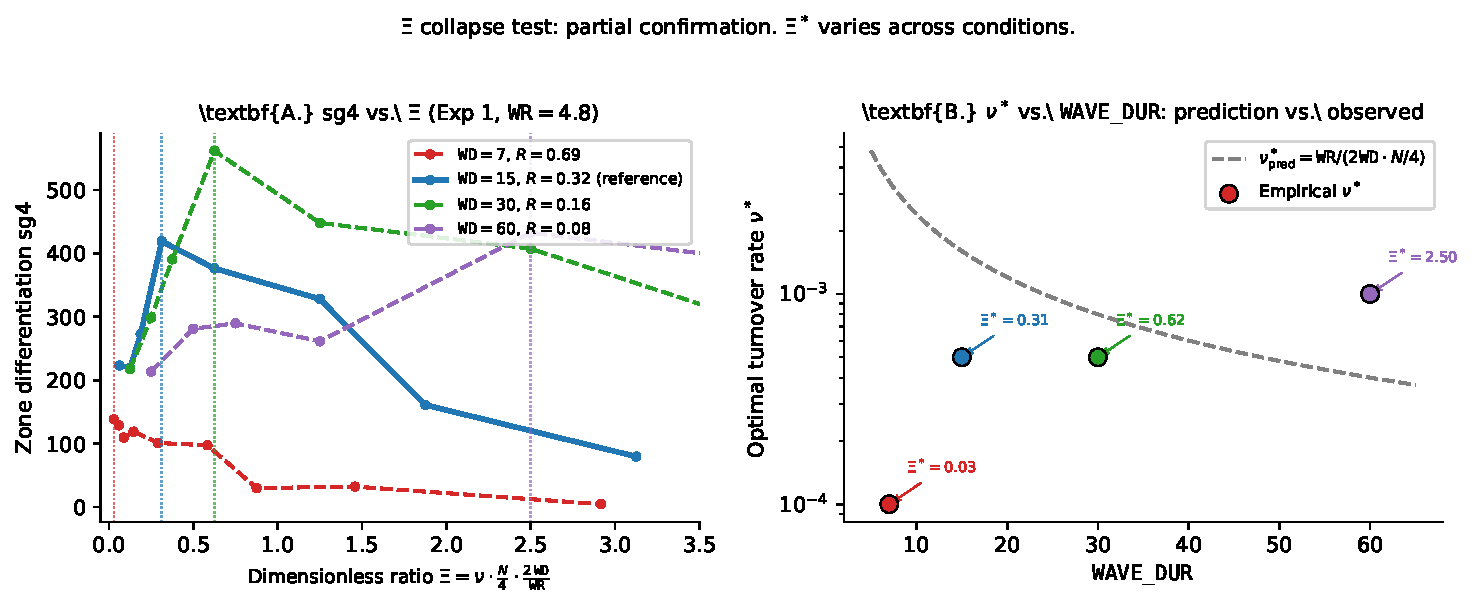
\includegraphics[width=\linewidth]{paper9_figure1}
\caption{\textbf{Testing the Xi collapse.}
\textbf{A}: $\mathtt{sg4}$ vs.\ $\Xi = \nu \cdot 100 \cdot 2\,\mathtt{WD}/\mathtt{WR}$
for Exp~1 (WAVE\_DUR sweep at $\mathtt{WR}=4.8$). Curves do not collapse: $\Xi^*$
varies from 0.029 (WD=7, over-perturbed) to 2.5 (WD=60, reversed).
\textbf{B}: Empirical $\nu^*$ vs.\ WAVE\_DUR with the prediction line from the
balance equation ($\nu^*_{\text{pred}} \propto 1/\mathtt{WD}$). Empirical values
do not follow the prediction (WD=60 goes in the wrong direction; WD=15,30 show
the same $\nu^*$ despite a $2\times$ WAVE\_DUR change).}
\label{fig:collapse}
\end{figure}

Figure~\ref{fig:collapse} Panel~A shows the non-collapse: the adaptive peaks
(vertical dotted lines) fall at different $\Xi$ values across WAVE\_DUR conditions.
Panel~B shows that the balance-equation prediction line ($\nu^*_{\text{pred}}
\propto 1/\mathtt{WD}$) overestimates the sensitivity of $\nu^*$ to WAVE\_DUR.

% ============================================================
\section{Interpretation: Why the Single Ratio Fails}
\label{sec:interp}

\subsection{Two Independent Effects}

The balance equation (Eq.~\eqref{eq:balance}) uses only the ratio
$R = \mathtt{WR}/\mathtt{WAVE\_DUR}$. The experiments reveal two additional
dependencies:

\textbf{Effect 1: Perturbation load ($P_{\text{pert}}$, depends on absolute WR).}
In VCML, perturbed sites age at twice the normal rate
($\mathtt{ttl}[i] \mathrel{-}= 1$ for all; additional $\mathtt{ttl}[\text{pert}]
\mathrel{-}= 1$). The effective death rate is $\nu_{\text{eff}} = \nu \cdot
(1 + P_{\text{pert}})$. At reference WR=4.8, $P_{\text{pert}} \approx 0.91$,
so $\nu_{\text{eff}} \approx 1.91\nu$. At WR=1.6, $\nu_{\text{eff}} \approx
1.55\nu$. The balance condition is reached at a lower nominal $\nu$ when
$P_{\text{pert}}$ is higher. This accounts for part of the ratio-collapse
failure in Exp~2.

\textbf{Effect 2: Consolidation probability ($P_{\text{calm}}$, depends on
absolute WAVE\_DUR and $R$).}
$P_{\text{calm}} \approx (1-R/2)^{SS+\mathtt{WD}-1}$. At fixed $R$, longer
WAVE\_DUR exponentially reduces $P_{\text{calm}}$: from 0.084 (WD=5) to
0.0013 (WD=30) for the pairs in Exp~2. This dramatically affects the amplitude
of $\mathtt{sg4}^*$ (Table~\ref{tab:exp2}: 206, 419, 403) and likely shifts
the balance condition for $\nu^*$ as well. With very low $P_{\text{calm}}$
(WD=30, WD=60), fewer sites contribute to the copy-forward balance per step,
requiring lower $\nu$ to maintain the equilibrium.

\subsection{A Corrected Picture}

The full balance condition is approximately:
\begin{equation}
  \nu_{\text{eff}} \cdot P_{\text{calm}} \;\approx\; \text{constant}
  \quad \Rightarrow \quad
  \nu \cdot (1 + P_{\text{pert}}) \cdot (1-R/2)^{SS+\mathtt{WD}-1}
    \;\approx\; \text{constant}
  \label{eq:corrected}
\end{equation}
This is no longer a simple function of $R$ alone: it depends on WR (via
$P_{\text{pert}}$) and on WAVE\_DUR (via the exponent $SS + \mathtt{WD} - 1$),
independently of their ratio. The regime boundary requires at least two
dimensionless quantities: a ratio ($R$) and a scale (e.g., $\mathtt{WR}$ or
$\mathtt{WD}$ individually).

The balance equation of Paper~8 is the limit of Eq.~\eqref{eq:corrected} when
$P_{\text{pert}} \ll 1$ (small WR) and $SS \gg \mathtt{WD}$ (consolidation gate
dominates over wave duration). In the reference condition (WR=4.8, WD=15,
$P_{\text{pert}} = 0.91$), neither limit holds, which is why the balance equation
worked only to within a factor of $\sim$2.

\subsection{Operational Range Interpretation}

The Paper~8 invariance ($\nu^*$ stable across $\kappa$, SS, FIELD\_ALPHA) holds
because those parameters do not appear in Eq.~\eqref{eq:corrected} at all.
They control amplitude ($\mathtt{sg4}^*$) via the pre-factor, but not the balance
point $\nu^*$. By contrast, WR and WAVE\_DUR appear in Eq.~\eqref{eq:corrected}
and \emph{do} shift $\nu^*$---they were simply not varied in Paper~8.

The hierarchy of governing parameters is:
\begin{center}
\begin{tabular}{lll}
\toprule
Parameter & Controls & Appears in $\nu^*$ condition? \\
\midrule
$\kappa$, SS, FIELD\_ALPHA & Amplitude only & No \\
$R = \mathtt{WR}/\mathtt{WAVE\_DUR}$ & Location (dominant term) & Yes \\
$\mathtt{WR}$ (via $P_{\text{pert}}$) & Location (second-order) & Yes \\
$\mathtt{WAVE\_DUR}$ (via $P_{\text{calm}}$ exponent) & Location (second-order) & Yes \\
\bottomrule
\end{tabular}
\end{center}

% ============================================================
\section{Discussion}

\subsection{The Single-Ratio Hypothesis Was Too Simple}

The $\Xi$ hypothesis captured the right variables (wave input dynamics) and the
right structure (a ratio of rates), but collapsed two independent effects into one.
The balance equation $\nu^* \approx R \cdot 2 / N_{\text{act}}$ is the correct
leading term but misses the perturbation-load correction from $P_{\text{pert}}$
and the consolidation-gate correction from $P_{\text{calm}}$.

This is the expected outcome for a first-order post-hoc estimate applied outside
its derivation range. The correction matters when $P_{\text{pert}}$ is not small
(WR $\gtrsim 1$) and when WAVE\_DUR is not much shorter than $1/R$ (i.e.,\ when
the burst structure of perturbations matters).

\subsection{What the Experiments Do Confirm}

\begin{enumerate}
  \item WAVE\_DUR and WR each have independent effects on $\nu^*$, as predicted
    by the corrected balance (Eq.~\eqref{eq:corrected}).
  \item Short WAVE\_DUR at high $R$ collapses the adaptive window (WD=7), exactly
    as high WR collapses it in Paper~8. The over-perturbation regime is symmetric
    in WR and WAVE\_DUR.
  \item The WAVE\_DUR=30 reference case gives $\Xi^* = 0.625$, matching the
    theoretical prediction from Paper~8's reference condition. The balance equation
    is accurate at the reference point; its failure emerges only when extrapolating.
  \item Amplitude ($\mathtt{sg4}^*$) is dramatically affected by WAVE\_DUR: from
    138.5 (WD=7) to 561.7 (WD=30), confirming that consolidation probability
    governs amplitude as expected.
\end{enumerate}

\subsection{Relation to the Three-Paper Series}

The series Papers~7--9 now provides a layered understanding of the adaptive regime:

\begin{enumerate}
  \item (Paper~7) The adaptive window exists: a four-regime structure in
    $(\nu, \kappa)$ space, robust to metric choice, ablation, and scaling.
  \item (Paper~8) The window location is invariant to parameters that do not
    appear in the wave-grid balance: $\kappa$, SS, FIELD\_ALPHA.
  \item (Paper~9) The window location \emph{does} respond to WR and WAVE\_DUR
    individually, beyond their ratio. The leading term (ratio $R$) and two
    correction terms ($P_{\text{pert}}$, $P_{\text{calm}}$ exponent) together
    describe the balance, requiring a future theoretical derivation to unify them.
\end{enumerate}

\subsection{Limitations}

The 5-seed count makes the WAVE\_DUR=60 profile unreliable (the non-monotone
dip at $\nu = 0.0005$ is likely noise). Future experiments should increase seeds
or run length for very long WAVE\_DUR, where equilibration may require $>2000$ steps.
The corrected balance (Eq.~\eqref{eq:corrected}) is still a heuristic; a
rigorous derivation from the VCSM update rule remains for future work.

% ============================================================
\section{Conclusion}

The single-ratio hypothesis ($\Xi = \nu \cdot 2\,\mathtt{WD} \cdot N/(4\,\mathtt{WR})$
governs the adaptive window) is not confirmed. $\Xi^*$ is not constant across
WAVE\_DUR conditions (Exp~1) and the ratio collapse fails when WR varies at fixed
$R$ (Exp~2). The failure identifies two independent effects missing from the
balance equation: the perturbation load $P_{\text{pert}}(WR)$ and the consolidation
probability $P_{\text{calm}}(R, \mathtt{WD})$. A corrected balance
(Eq.~\eqref{eq:corrected}) involves both, requiring at least two dimensionless
quantities to characterize the regime boundary.

The positive contributions of the paper are the identification of those two
missing terms and the confirmation that WR and WAVE\_DUR have independent effects
--- a more complete characterization of what governs the adaptive regime than
was available after Paper~8. The invariances of Paper~8 are fully consistent
with this picture: the parameters that are invariant ($\kappa$, SS, FIELD\_ALPHA)
genuinely do not appear in the corrected balance condition.

% ============================================================
\appendix
\section{Reproducibility}

\begin{center}
\begin{tabular}{lll}
\toprule
Script & Description & Runtime \\
\midrule
\texttt{paper9\_exp1\_wave\_dur\_sweep.py} & WAVE\_DUR sweep (240 runs) & $\sim$12 min \\
\texttt{paper9\_exp2\_ratio\_collapse.py}  & Ratio collapse (180 runs)  & $\sim$10 min \\
\texttt{paper9\_figure1\_xi\_collapse.py}  & Figure (Exp~1 cached data) & $<$1 min \\
\bottomrule
\end{tabular}
\end{center}

\begin{lstlisting}[caption={Run experiments and generate figure.}]
cd papers/paper9_governing_ratio
py paper9_exp1_wave_dur_sweep.py
py paper9_exp2_ratio_collapse.py
py paper9_figure1_xi_collapse.py
\end{lstlisting}

\end{document}
